\exercisesection

\begin{exercise} \label{exercise 6.3.1}
Label the following statements as true or false.
Assume that the underlying inner product spaces are \textbf{finite}-dimensional.
\begin{enumerate}
\item Every linear operator has an adjoint.
\item Every linear operator on \(\V\) has the form \(x \to \LG x, y \RG\) for some \(y \in \V\).
\item For every linear operator \(\T\) on \(\V\) and every ordered basis \(\beta\) for \(\V\), we have \([\T^*]_{\beta} = ([\T]_{\beta})^*\).
\item The adjoint of a linear operator is unique.
\item For any linear operators \(\T\) and \(\U\) and scalars \(a\) and \(b\),
\[
    (a\T + b\U)^* = a\T^*+ b\U^*.
\]
\item For any \(n \X n\) matrix \(A\), we have \((\LMTRAN_A)^* = \LMTRAN_{A^*}\).
\item For any linear operator \(\T\), we have \((\T^*)^* = \T\).
\end{enumerate}
\end{exercise}

\begin{proof} \ 

\begin{enumerate}
\item True by \THM{6.9}.
\item False. Only linear \emph{transformation} from \(\V\) to \(F\) has the form \(x \to \LG x, y \RG\) for some \(y \in \V\) by \THM{6.8}.
\item False. \(\beta\) also needs to be \emph{orthonormal}; see \THM{6.10}.
Counterexample, \(\T = \LMTRAN_A\) where \(A = \begin{pmatrix} 1 & 1 \\ 0 & 1 \end{pmatrix}\), then in particular, by \CORO{6.10.1}, \(\T^* = \LMTRAN_{A^*}\).
But with a (non-orthonormal) basis \(\beta = \{(1, 1), (0, 1)\}\), we have
\[
    ([\T]_{\beta}) = \begin{pmatrix} 2 & 1 \\ -1 & 0 \end{pmatrix} \text{ hence } ([\T]_{\beta})^* = \begin{pmatrix} 2 & -1 \\ 1 & 0 \end{pmatrix} \text{\quad and \quad} [\T^*]_{\beta} = \begin{pmatrix} 1 & 0 \\ 1 & 1 \end{pmatrix}
\]
Hence \THM{6.10} does not apply when the basis is not orthonormal.

\item True by \THM{6.9}.
\item False,
we have
\begin{align*}
    (a\T + b\U)^* & = (a\T)^* + (b\U)^* & \text{by \THM{6.11}(a)} \\
        & = \conjugatet{a}\T^* + \conjugatet{b}\U^* & \text{by \THM{6.11}(b)}
\end{align*}
\item True by \CORO{6.10.1}.
\item True by \THM{6.11}(d).
\end{enumerate}
\end{proof}

\begin{exercise} \label{exercise 6.3.2}
For each of the following inner product spaces \(\V\) (over \(F\)) and \LTRAN{}s \(g : \V \to F\), find a vector \(y\) such that \(g(x) = \LG x, y \RG\) for all \(x \in \V\).
\begin{enumerate}
\item \(\V = \SET{R}^3\), \(g(a_1, a_2, a_3) = a_1 - 2a_2 + 4a_3\)
\item \(\V = \SET{C}^2\), \(g(z_1, z_2) = z_1 - 2z_2\)
\item \(\V = \POLYRR\) with \(\LG f(x), h(x) \RG = \int_0^1 f(t)h(t) dt\), and \(g(f) = f(0) + f'(1)\)
\end{enumerate}
\end{exercise}

\begin{proof} \ 
Note that by the description in the proof of \THM{6.8}, given any orthonormal basis \(\beta = \{ v_1, ..., v_n \}\) for \(\V\), the desired \(y\) has the form
\[
    y = \sum_{i = 1}^n \conjugatet{g(v_i)}v_i. \quad \quad \MAROON{(1)}
\]

\begin{enumerate}
\item Let \(\beta = \{ e_1, e_2, e_3 \}\) be the standard ordered (orthonormal) basis for \(\SET{R}^3\).
Then
\begin{align*}
    y & = g(e_1)e_1 + g(e_2)e_2 + g(e_3)e_3 & \text{by \MAROON{(1)} but now \(F = \SET{R}\)} \\
      & = 1 \cdot e_1 + -2 \cdot e_2 + 4 \cdot e_3 = (1, -2, 4).
\end{align*}

\item Let \(\beta = \{ e_1, e_2 \}\) be the standard ordered (orthonormal) basis for \(\SET{C}^2\).
Then
\begin{align*}
    y & = \conjugatet{g(e_1)}e_1 + \conjugatet{g(e_2)}e_2 & \text{by \MAROON{(1)}} \\
      & = \conjugatet{1} \cdot e_1 + \conjugatet{-2} \cdot e_2 = (1, -2).
\end{align*}

\item We should first deduce an orthonormal basis for the inner product space; the problem is the same as \EXEC{6.2.2}(c), but I have skipped that problem.
Using Gram-Schmidt process and normalizing the result, we have an orthonormal basis
\[
    \beta = \{ b_1, b_2, b_3 \} = \left\{ 1, 2\sqrt{3} \left( t - \frac{1}{2} \right), 6\sqrt{5} \left( t^2 - t + \frac{1}{6} \right) \right\}.
\]
And
\begin{align*}
    g(b_1) & = b_1(0) + b_1'(1) = 1 + 0 = 1 \\
    g(b_2) & = b_2(0) + b_2'(1) = -\sqrt{3} + 2\sqrt{3} = \sqrt{3} \\
    g(b_3) & = b_3(0) + b_3'(1) = \sqrt{5} + 6\sqrt{5} = 7\sqrt{5}
\end{align*}
Hence
\begin{align*}
    y & = g(b_1) b_1 + g(b_2) b_2 + g(b_3) b_3 & \text{by \MAROON{(1)} but now \(F = \SET{R}\)} \\
      & = 1 \cdot 1 + \sqrt{3} \cdot 2\sqrt{3} \left( t - \frac{1}{2} \right) + 7\sqrt{5} \cdot 6\sqrt{5} \left( t^2 - t + \frac{1}{6} \right) \\
      & = 33 - 204t + 210t^2.
\end{align*}
\end{enumerate}
\end{proof}

\begin{exercise} \label{exercise 6.3.3}
For each of the following inner product spaces \(\V\) and linear operators \(\T\) on \(\V\), evaluate \(\T^*\) at the given vector in \(\V\).
\begin{enumerate}
\item \(\V = \SET{R}^2\), \(\T(a, b) = (2a + b, a - 3b)\), \(x = (3, 5)\).
\item \(\V = \SET{C}^2\), \(\T(z_1, z_2) = (2z_1 + \iu z_2, (1 - \iu)z_1)\), \(x = (3 - \iu, 1 + 2\iu)\).
\item \(\V = \POLYR\) with \(\LG f(x),g(x) \RG = \int_{-1}^1 f(t) g(t) dt\), \(\T(f) = f' + 3f\), \(f(t) = 4 - 2t\).
\end{enumerate}
\end{exercise}

\begin{proof} \ 

\begin{enumerate}
\item Let \(\beta = \{ e_1, e_2 \}\) be the standard ordered (orthonormal) basis for \(\SET{R}^2\).
Then
\begin{align*}
    [\T]_{\beta} & = \begin{pmatrix} 2 & 1 \\ 1 & -3 \end{pmatrix} & \text{of course} \\
    \implies & [\T^*]_{\beta} = ([\T]_{\beta})^* = \begin{pmatrix} 2 & 1 \\ 1 & -3 \end{pmatrix}^* = \begin{pmatrix} 2 & 1 \\ 1 & -3 \end{pmatrix} & \text{by \THM{6.10}}
\end{align*}
(In particular, \(\T\) is \emph{self-adjoint}, see \DEF{6.9}.)
Then from the matrix representation of \([\T^*]_{\beta}\), we have \(\T^*(a, b) = (2a + b, a - 3b)\); and for \(x = (3, 5)\), \(\T^*(3, 5) = (2 \cdot 3 + 5, 3 - 3 \cdot 5) = (11, -12)\).

\item Let \(\beta = \{ e_1, e_2 \}\) be the standard ordered (orthonormal) basis for \(\SET{C}^2\).
Then
\begin{align*}
    [\T]_{\beta} & = \begin{pmatrix} 2 & \iu \\ 1 - \iu & 0 \end{pmatrix} & \text{of course} \\
    \implies & [\T^*]_{\beta} = ([\T]_{\beta})^* = \begin{pmatrix} 2 & \iu \\ 1 - \iu & 0 \end{pmatrix}^* = \begin{pmatrix} 2 & 1 + \iu \\ -\iu & 0 \end{pmatrix} & \text{by \THM{6.10}}
\end{align*}
Then from the matrix representation of \([\T^*]_{\beta}\), we have \(\T^*(z_1, z_2) = (2z_1 + (1 + \iu)z_2, -z_1)\); and for \(x = (3 - \iu, 1 + 2\iu)\), \(\T^*(3 - \iu, 1 + 2\iu) = (5 + \iu, -1 - 3\iu)\).

\item Using Gram-Schmidt process and normalizing the result, we have an orthonormal basis
\[
    \beta = \left\{ \frac{1}{\sqrt{2}}, \sqrt{\frac{3}{2}} \cdot t \right\}
\]
In particular,
\begin{align*}
    \T \left( \frac{1}{\sqrt{2}} \right)
        & = \left(\frac{1}{\sqrt{2}}\right)' + 3 \cdot \frac{1}{\sqrt{2}} = \frac{3}{\sqrt{2}} \\
        & = 3 \cdot \frac{1}{\sqrt{2}} + 0 \cdot \sqrt{\frac{3}{2}} \cdot t, \\
    \T \left( \sqrt{\frac{3}{2}} \cdot t \right)
        & = \left(\sqrt{\frac{3}{2}} \cdot t \right)' + 3 \cdot \sqrt{\frac{3}{2}} \cdot t = \sqrt{\frac{3}{2}} + 3\sqrt{\frac{3}{2}} \cdot t \\
        & = \sqrt{3} \cdot \frac{1}{\sqrt{2}} + 3 \cdot \sqrt{\frac{3}{2}} \cdot t
\end{align*}
Hence \([\T]_{\beta} = \begin{pmatrix} 3 & \sqrt{3} \\ 0 & 3 \end{pmatrix}\), and by \THM{6.10}, \([\T^*]_{\beta} = ([\T]_{\beta})^* = \begin{pmatrix} 3 & \sqrt{3} \\ 0 & 3 \end{pmatrix}^* = \begin{pmatrix} 3 & 0 \\ \sqrt{3} & 3 \end{pmatrix}\).
Now note that for \(f(t) = 4 - 2t\), (by calculation) \([f(t)]_{\beta} = \begin{pmatrix} \frac{8}{\sqrt{2}} \\ -\frac{2\sqrt{2}}{\sqrt{3}} \end{pmatrix}\), and
\begin{align*}
    [\T^*(f(t))]_{\beta} & = [\T^*]_{\beta} [f(t)]_{\beta} & \text{by \THM{2.14}} \\
        & = \begin{pmatrix} 3 & 0 \\ \sqrt{3} & 3 \end{pmatrix} \begin{pmatrix} \frac{8}{\sqrt{2}} \\ -\frac{2\sqrt{2}}{\sqrt{3}} \end{pmatrix} \\
        & = \begin{pmatrix} \frac{24}{\sqrt{2}} \\ \frac{8\sqrt{3}}{\sqrt{2}} - \frac{6\sqrt{2}}{\sqrt{3}} \end{pmatrix},
\end{align*}
which implies (by calculation) \(\T^*(f(t)) = 12 + 6t\).
\end{enumerate}
\end{proof}

\begin{exercise} \label{exercise 6.3.4}
Complete the proof of \THM{6.11}.
\end{exercise}

\begin{proof}
See \THM{6.11}.
\end{proof}

\begin{exercise} \label{exercise 6.3.5} \ 

\begin{enumerate}
\item Complete the proof of the \CORO{6.11.1} by using \THM{6.11}, as in the proof of (c).
\item State a result for \textbf{nonsquare} matrices that is analogous to the \CORO{6.11.1}, and prove it using a matrix argument.
\end{enumerate}
\end{exercise}

\begin{proof} \ 

\begin{enumerate}
\item See \CORO{6.11.1}.

\item The statement is:

Let \(A\) and \(B\) be \(m \X n\) matrices, \(C\) be \(n \X p\) matrix.
Then
\begin{enumerate}
\item \((A + B)^* = A^* + B^*\).
\item \((cA)^* = \conjugatet{c}A^*\) for all \(c \in F\).
\item \((AC)^* = C^*A^*\).
\item \(A^{**} = A\).
(Precisely, \(A^{**}\) is just \((A^*)^*\).)
\end{enumerate}
Note that there is no statement corresponding to \CORO{6.11.1}(e), since there is no ``identity'' nonsquare matrix.
\begin{proof} \

\begin{enumerate}
\item We have for all \(i, j\) where \(1 \le i \le m\) and \(1 \le j \le n\),
\begin{align*}
    (A + B)^*_{ij} & = \conjugatet{(A + B)_{ji}} & \text{by \DEF{6.2}} \\
        & = \conjugatet{A_{ji} + B_{ji}} & \text{by def of matrix \(+\)} \\
        & = \conjugatet{A_{ji}} + \conjugatet{B_{ji}} & \text{by \THM{d.2}(b)} \\
        & = A^*_{ij} + B^*_{ij} & \text{by \DEF{6.2}} \\
        & = (A^* + B^*)_{ij} & \text{by def of matrix \(+\)}
\end{align*}
Hence \((A + B)^* = A^* + B^*\).

\item We have for all \(i, j\) where \(1 \le i \le m\) and \(1 \le j \le n\),
\begin{align*}
    (cA)^*_{ij} & = \conjugatet{(cA)_{ji}} & \text{by \DEF{6.2}} \\
        & = \conjugatet{c \cdot A_{ji}} & \text{by def of matrix scalar \(\cdot\)} \\
        & = \conjugatet{c} \cdot \conjugatet{A_{ji}} & \text{by \THM{d.2}(c)} \\
        & = \conjugatet{c} \cdot A^*_{ij} & \text{by \DEF{6.2}} \\
        & = (\conjugatet{c} A^*)_{ij} & \text{by def of matrix scalar \(\cdot\)}
\end{align*}
Hence \((cA)^* = \conjugatet{c}A^*\).

\item We have for all \(i, j\) where \(1 \le i \le \RED{p}\) and \(1 \le j \le \RED{m}\).
\begin{align*}
    (AC)^*_{ij} & = \conjugatet{(AC)_{ji}} & \text{by \DEF{6.2}} \\
        & = \conjugatet{\sum_{k = 1}^n A_{jk}C_{ki}} & \text{by def of matrix product} \\
        & = \sum_{k = 1}^n \conjugatet{A_{jk}C_{ki}} & \text{by \THM{d.2}(b)} \\
        & = \sum_{k = 1}^n \conjugatet{A_{jk}} \cdot \conjugatet{C_{ki}} & \text{by \THM{d.2}(c)} \\
        & = \sum_{k = 1}^n A^*_{kj} C^*_{ik} = \sum_{k = 1}^n C^*_{ik} A^*_{kj} & \text{by \DEF{6.2}} \\
        & = (C^* A^*)_{ij} & \text{by def of matrix product}
\end{align*}
Hence \((AC)^* = C^*A^*\).

\item
We have for all \(i, j\) where \(1 \le i \le m\) and \(1 \le j \le n\),
\begin{align*}
    (A^{**})_{ij} & = \conjugatet{A^*_{ji}} & \text{by \DEF{6.2}} \\
        & = \conjugatet{\conjugatet{A_{ij}}} & \text{by \DEF{6.2} again} \\
        & = A_{ij} & \text{by \THM{d.2}(a)}
\end{align*}
Hence \(A^{**} = A\).
\end{enumerate}
\end{proof}

\end{enumerate}
\end{proof}

\begin{exercise} \label{exercise 6.3.6}
Let \(\T\) be a linear operator on an inner product space \(\V\).
Let \(\U_1 = \T + \T^*\) and \(\U_2 = \T\T^*\).
Prove that \(\U_1 = \U_1^*\) and \(\U_2 = \U_2^*\).
\end{exercise}

\begin{note}
These are some examples of self-adjoint (see \DEF{6.9}) operators.
\end{note}

\begin{proof}
We have
\begin{align*}
    \U_1^* & = (\T + \T^*)^* \\
        & = \T^* + (\T^*)^* & \text{by \THM{6.11}(a)} \\
        & = \T^* + \T = \T + \T^* = \U_1 & \text{by \THM{6.11}(d)}
\end{align*}
and
\begin{align*}
    \U_2^* & = (\T\T^*)^* \\
        & = (\T^*)^* \T^* & \text{by \THM{6.11}(c)} \\
        & = \T\T^* = \U_2, & \text{by \THM{6.11}(d)}
\end{align*}
So \(\U_1^* = \U_1\) and \(\U_2^* = \U_2\), as desired.
\end{proof}

\begin{exercise} \label{exercise 6.3.7}
Give an example of a linear operator \(\T\) on an inner product space \(\V\) such that \(\NULLT \ne \NULL(\T^*)\).
\end{exercise}

\begin{proof}
Let \(A = \begin{pmatrix} 1 & 1 \\ 0 & 0 \end{pmatrix}\), and let \(\T = \LMTRAN_A\), hence \(\T^* = (\LMTRAN_A)^* = \LMTRAN_{A^*}\) by \THM{6.10}.
But we have
\[
    \T(0, 1) = (1, 0), \T^*(0, 1) = (0, 0)
\]
Hence \((0, 1) \notin \NULLT\) but \((0, 1) \in \NULL(\T^*)\), hence \(\NULLT \ne \NULL(\T^*)\).
\end{proof}

\begin{exercise} \label{exercise 6.3.8}
Let \(\V\) be a finite-dimensional inner product space, and let \(\T\) be a linear operator on \(\V\).
Prove that if \(\T\) is invertible, then \(\T^*\) is invertible and \((\T^*)^{-1} = (\T^{-1})^*\).
\end{exercise}

\begin{note}
給定一個可逆變換\ \(\T\),\(\T\) 的\ adjoint 的\ inverse 等於\ \(\T\) 的\ inverse 的\ adjoint。
\end{note}

\begin{proof}
Suppose \(\T\) is invertible, hence \(\T^{-1}\) and \((\T^{-1})^*\) exists.
And
\begin{align*}
    \T^* (\T^{-1})^* & = (\T^{-1} \T)^* & \text{by \THM{6.11}(c)} \\
        & = \ITRAN{}^* & \text{of course} \\
        & = \ITRAN{} & \text{by \THM{6.11}(e)}
\end{align*}
and
\begin{align*}
    (\T^{-1})^* \T^* & = (\T \T^{-1})^* & \text{by \THM{6.11}(c)} \\
        & = \ITRAN{}^* & \text{of course} \\
        & = \ITRAN{} & \text{by \THM{6.11}(e)}
\end{align*}
Hence by \DEF{2.12}, \(\T^*\) is invertible and its inverse is \((\T^{-1})^*\), that is, \((\T^*)^{-1} = (\T^{-1})^*\).
\end{proof}

\begin{exercise} \label{exercise 6.3.9}
Prove that if \(\V = \W \oplus \W^{\perp}\) and \(\T\) is the \emph{projection} on \(\W\) along \(\W^{\perp}\), then \(\T = \T^*\).
\emph{Hint}: Recall that \(\NULLT = \W^{\perp}\) (by \EXEC{2.1.27}(b)).
\end{exercise}

\begin{note}
So being a projection operator is a sufficient condition to be self-adjoint(see \DEF{6.9}) operator.
\end{note}

\begin{remark} \label{remark 6.3.8}
From this section, if we want to prove any two operators \(\T_1, \T_2\) on an inner product space \(\V\) are the same, we often prove that \(\LG x, \T_1(y) \RG = \LG x, \T_2(y) \RG\) for all \(x, y \in \V\), then by \THM{6.1}(e), \(\T_1(y) = \T_2(y)\) for all \(y \in \V\), hence \(\T_1 = \T_2\).
\end{remark}

\begin{proof}
Let \(x, y\) be arbitrary vectors in \(\V\), where \(x = a_1 + a_2, y = b_1 + b_2\) and \(a_1, b_1 \in \W, a_2, b_2 \in \W^{\perp}\).
Then
\begin{align*}
    \LG x, \T(y) \RG & = \LG a_1 + a_2, \T(b_1 + b_2) \RG \\
        & = \LG a_1 + a_2, b_1 \RG & \text{since \(\T\) is a projection} \\
        & = \LG a_1, b_1 \RG + \LG a_2, b_1 \RG & \text{by \DEF{6.1}(a)} \\
        & = \LG a_1, b_1 \RG + 0 & \text{since \(a_2, b_1\) are orthogonal} \\
        & = \LG a_1, b_1 \RG.
\end{align*}
and
\begin{align*}
    \LG x, \T^*(y) \RG & = \LG a_1 + a_2, \T^*(b_1 + b_2) \RG \\
        & = \LG \T(a_1 + a_2), b_1 + b_2 \RG & \text{by \THM{6.9}} \\
        & = \LG a_1, b_1 + b_2 \RG & \text{since \(\T\) is a projection} \\
        & = \LG a_1, b_1 \RG + \LG a_1, b_2 \RG & \text{by \THM{6.1}(a)} \\
        & = \LG a_1, b_1 \RG + 0 & \text{since \(a_1, b_2\) are orthogonal} \\
        & = \LG a_1, b_1 \RG = \LG x, \T(y) \RG & \text{by what we have shown}
\end{align*}
Hence by \THM{6.1}(e), \(\T(y) = \T^*(y)\) for all \(y \in \V\), hence \(\T = \T^*\).
\end{proof}

\begin{exercise} \label{exercise 6.3.10}
Let \(\T\) be a linear operator on an inner product space \(\V\).
Prove that \(\norm{\T(x)} = \norm{x}\) for all \(x \in \V\) if and only if \(\LG \T(x), \T(y) \RG = \LG x, y \RG\) for all \(x, y \in \V\).
\emph{Hint}: Use \EXEC{6.1.20}.
\end{exercise}

\begin{note}
\THM{6.18} has some similar statements.
\end{note}

\begin{proof} \ 

\(\Longleftarrow\): Suppose \(\LG \T(x), \T(y) \RG = \LG x, y \RG\) for all \(x, y \in \V\).
In particular, \(\LG \T(x), \T(x) \RG = \LG x, x \RG\) for all \(x \in \V\), that is, by \DEF{6.3}, \(\norm{\T(x)}^2 = \norm{x}^2\) for all \(x \in \V\), which implies (since norm is nonnegative,) \(\norm{\T(x)} = \norm{x}\) for all \(x \in \V\), as desired.

\(\Longrightarrow\): Suppose \(\norm{\T(x)} = \norm{x}\) for all \(x \in \V\).

If \(\V\) is over \(\SET{R}\), then for all \(x, y \in \V\),
\begin{align*}
    4 \LG \T(x), \T(y) \RG & = \norm{\T(x) + \T(y)}^2 - \norm{\T(x) - \T(y)}^2 & \text{by \EXEC{6.1.20}(a)} \\
        & = \norm{\T(x + y)}^2 - \norm{\T(x - y)}^2 & \text{since \(\T\) is linear} \\
        & = \norm{x + y}^2 - \norm{x - y}^2 & \text{by supposition} \\
        & = \LG x + y, x + y \RG - \LG x - y, x - y \RG & \text{by \DEF{6.3}} \\
        & = (\LG x, x \RG + \LG x, y \RG + \LG y, x \RG + \LG y, y \RG) \\
        & \quad - (\LG x, x \RG - \LG x, y \RG - \LG y, x \RG + \LG y, y \RG) & \text{by \DEF{6.1} \THM{6.1}(a)(b)} \\
        & = 2 \LG x, y \RG + 2 \LG y, x \RG & \text{of course} \\
        & = 2 \LG x, y \RG + 2 \LG x, y \RG = 4 \LG x, y \RG & \text{since \(F = \SET{R}\)} \\
    \implies & \LG \T(x), \T(y) \RG = \LG x, y \RG.
\end{align*}

If \(\V\) is over \(\SET{C}\), then the proof is similar using \EXEC{6.1.20}(b), although tedious:
\begin{align*}
    & 4 \LG \T(x), \T(y) \RG \\
    & = \iu^1 \norm{\T(x) + \iu^1 \T(y)}^2 + \iu^2 \norm{\T(x) + \iu^2 \T(y)}^2
        + \iu^3 \norm{\T(x) + \iu^3 \T(y)}^2 + \iu^4 \norm{\T(x) + \iu^4 \T(y)}^2 \\
        & \text{\quad \quad \quad (by \EXEC{6.1.20}(b))} \\
    & = \iu \norm{\T(x) + \iu \T(y)}^2
        - \norm{\T(x) - \T(y)}^2
        - \iu\norm{\T(x) - \iu \T(y)}^2 + \norm{\T(x) + \T(y)}^2 \\
        & \text{\quad \quad \quad (of course)} \\
    & = \iu \norm{\T(x + \iu y)}^2
        - \norm{\T(x - y)}^2
        - \iu\norm{\T(x - \iu y)}^2 + \norm{\T(x + y)}^2 \\
        & \text{\quad \quad \quad (since \(\T\) is linear)} \\
    & = \iu \norm{x + \iu y}^2
        - \norm{x - y}^2
        - \iu\norm{x - \iu y}^2 + \norm{x + y}^2 \\
        & \text{\quad \quad \quad (by supposition that \(\norm{\T(x)} = \norm{x}\) for all \(x \in \V\)} \\
    & = \iu \LG x + \iu y, x + \iu y \RG
        - \LG x - y, x - y \RG
        - \iu \LG x - \iu y, x - \iu y \RG + \LG x + y, x + y \RG \\
        & \text{\quad \quad \quad (by \DEF{6.3})} \\
    & = ... = 4 \LG x, y \RG \\
    & \text{\quad \quad \quad (by brute force and tedious calculation)} \\
    \implies & \LG \T(x), \T(y) \RG = \LG x, y \RG.
\end{align*}

So for \(F = \SET{R}\) and \(F = \SET{C}\), we have \(\LG \T(x), \T(y) \RG = \LG x, y \RG\), as desired.
\end{proof}

\begin{exercise} \label{exercise 6.3.11}
For a linear operator \(\T\) on an inner product space \(\V\), prove that \(\T^*\T = \TZERO\) implies \(\T = \TZERO\).
Is the same result true if we assume that \(\T\T^* = \TZERO\)?
\end{exercise}

\begin{note}
若\ \(\T^*\T\) 是零函數,則\ \(\T\) 其實就是零函數。
\end{note}

\begin{proof}
By \RMK{6.3.4}, again we assume the existence of \(\T^*\).

We use the strategy in \RMK{6.3.8}.
For all \(x, y \in \V\),
\begin{align*}
    \LG x, \TZERO(v) \RG & = \LG x, \T^*\T(y) \RG & \text{by supposition} \\
        & = \LG \T(x), \T(y) \RG, & \text{by \THM{6.9}}
\end{align*}
which implies \(\LG \T(x), \T(y) \RG = 0\) for all \(x, y \in \V\).
In particular, we have \(\LG \T(x), \T(x) \RG = 0\) for all \(x \in \V\), that is, by \THM{6.1}(d), \(\T(x) = \OV\) for all \(x \in \V\), hence \(\T = \TZERO\).

For the second part, if \(\T\T^* = \TZERO\), then in particular, \(\T = \T^{**}\) by \THM{6.11}(d), hence we have \(\T^{**} \T^* = \TZERO\), that is, \((\T^*)^* \T^* = \TZERO\).
Then by the first part of the prove, we have \(\T^* = \TZERO\), but of course \(\TZERO = \TZERO^*\), hence \(\T^* = \TZERO^*\), hence (\(\T^{**} = \TZERO^{**}\) and) \(\T = \TZERO\).
\end{proof}

\begin{exercise} \label{exercise 6.3.12}
Let \(\V\) be an inner product space, and let \(\T\) be a linear operator on \(\V\).
Prove the following results.
\begin{enumerate}
\item \(\RANGE(\T^*)^{\perp} = \NULLT\).
\item If \(\V\) is \textbf{finite}-dimensional, then \(\RANGE(\T^*) = \NULLT^{\perp}\).
\emph{Hint}: Use \EXEC{6.2.13}(c).
\end{enumerate}
\end{exercise}

\begin{proof} \ 

\begin{enumerate}
\item We show \(\RANGE(\T^*)^{\perp} \subseteq \NULLT\) and \(\NULLT \subseteq \RANGE(\T^*)^{\perp}\).

So suppose \(x \in \RANGE(\T^*)^{\perp}\).
Then by \DEF{6.7}, we have \(\LG x, y \RG = 0\) for all \(y \in \RANGE(\T^*)\), that is, \(\LG x, \T^*(x') \RG = 0\) for all \(x' \in \V\).
But by \THM{6.9}, \(\LG x, \T^*(x') \RG = \LG \T(x), x' \RG\), hence we have \(\LG \T(x), x' \RG = 0\) (and of course, \(\LG x', \T(x) \RG = 0\)) for all \(x' \in \V\).
So by \THM{6.1}(e), \(\T(x) = \OV\).
So by definition \(x \in \NULLT\), hence \(\RANGE(\T^*)^{\perp} \subseteq \NULLT\).

Now suppose \(x \in \NULLT\).
Then in particular, \(\T(x) = \OV\), so \(\LG \T(x), y \RG = 0\) for all \(y \in \V\).
Again by \THM{6.9}, \(\LG x, \T^*(y) \RG = 0\) for all \(y \in \V\), that is, \(\LG x, y' \RG = 0\) for all \(y' \in \RANGE(\T^*)\).
So by \DEF{6.7}, \(x \in \RANGE(\T^*)^{\perp}\), hence \(\NULLT \subseteq \RANGE(\T^*)^{\perp}\).

\item Since \(\V\) is finite-dimensional, by \EXEC{6.2.13}(c), \((\RANGE(\T^*)^{\perp})^{\perp} = \RANGE(\T^*)\) \MAROON{(1)}, and we have
\begin{align*}
    & \RANGE(\T^*)^{\perp} = \NULLT & \text{by part(a)} \\
    \implies & (\RANGE(\T^*)^{\perp})^{\perp} = \NULLT^{\perp} & \text{of course} \\
    \implies & \RANGE(\T^*) = \NULLT^{\perp}. & \text{by \MAROON{(1)}}
\end{align*}
\end{enumerate}
\end{proof}

\begin{exercise} \label{exercise 6.3.13}
Let \(\T\) be a linear operator on a \emph{finite}-dimensional inner product space \(\V\).
Prove the following results.
\begin{enumerate}
\item \(\NULL(\T^*\T) = \NULLT\).
Deduce that \(\rank(\T^*\T) = \rankT\).
\item \(\rankT = \rank(\T^*)\).
Deduce from (a) that \(\rank(\T\T^*) = \rankT\).
\item For any \(n \X n\) matrix \(A\), \(\rank(A^*A) = \rank(AA^*) = \rank(A)\).
\end{enumerate}
\end{exercise}

\begin{note}
Related lemma: \LEM{6.2}.
\end{note}

\begin{proof} \ 

\begin{enumerate}
\item If \(x \in \NULLT\) then \(\T(x) = \OV\), and \(\T^*\T(x) = \T^*(\T(x)) = \T^*(\OV) = \OV\), hence \(x \in \NULL(\T^*\T)\), so \(\NULLT \subseteq \NULL(\T^*\T)\).

If \(x \in \NULL(\T^*\T)\), then \(\T^*\T(x) = \OV\). \MAROON{(1)}

In particular,
\begin{align*}
    0 & = \LG x, \OV \RG & \text{by \THM{6.1}(c)} \\
      & = \LG x, \T^*\T(x) \RG & \text{by \MAROON{(1)}} \\
      & = \LG \T(x), \T(x), \RG & \text{by \THM{6.9}}
\end{align*}
which by \THM{6.1}(d) implies \(\T(x) = \OV\), hence \(x \in \NULLT\), so \(\NULL(\T^*\T) \subseteq \NULLT\).

So we have \(\NULL(\T^*\T) = \NULLT\) \MAROON{(2)}, and
\begin{align*}
    \rank(\T^*\T) & = \dim(\V) - \nullity(\T^*\T) & \text{by \THM{2.3}, dimension} \\
        & = \dim(\V) - \nullityT & \text{by \MAROON{(2)}} \\
        & = \rankT, & \text{by \THM{2.3}}
\end{align*}
as desired.

\item We have
\begin{align*}
    \rankT & = \dim(\V) - \nullityT & \text{by \THM{2.3}} \\
        & = \dim(\V) - \dim(\NULLT) & \text{by definition} \\
        & = \dim(\NULLT^{\perp}) & \text{by \THM{6.7}(c)} \\
        & = \dim(\RANGE(\T^*)) & \text{by \EXEC{6.3.12}(b)} \\
        & = \rank(\T^*) & \text{by definition}
\end{align*}
And in particular,
\begin{align*}
    \rank(\T \T^*) & = \rank((\T^*)^* \T^*) & \text{by \THM{6.11}(d)} \\
        & = \rank(\T^*). & \text{by part(a)}
\end{align*}

\item We have
\begin{align*}
    \rank(A) & = \rank(\LMTRAN_A) & \text{by \DEF{3.3}} \\
        & = \rank((\LMTRAN_A)^* \LMTRAN_A) = \rank(\LMTRAN_A (\LMTRAN_A)^*) & \text{by part(a) and (b)} \\
        & = \rank(\LMTRAN_{A^*} \LMTRAN_A) = \rank(\LMTRAN_A \LMTRAN_{A^*}) & \text{by \CORO{6.10.1}} \\
        & = \rank(\LMTRAN_{A^* A}) = \rank(\LMTRAN_{A A^*}) & \text{by \THM{2.15}(e)} \\
        & = \rank(A^* A) = \rank(A A^*) & \text{by \DEF{3.3}}
\end{align*}
\end{enumerate}
\end{proof}

\begin{exercise} \label{exercise 6.3.14}
Let \(\V\) be an inner product space, and let \(y, z \in \V\).
Define \(\T : \V \to \V\) by \(\T(x) = \LG x, y \RG z\) for all \(x \in \V\).
First prove that \(\T\) is linear.
Then show that \(\T^*\) \emph{exists}, and find an explicit expression for it.
\end{exercise}

\begin{note}
We do not say that \(\V\) is finite dimensional.
In particular, we cannot use \THM{6.8}.
\end{note}

\begin{proof}
Let \(x_1, x_2 \in \V\), \(c\) be scalar.
Then
\begin{align*}
    \T(c x_1 + x_2) & = \LG c x_1 + x_2, y \RG z & \text{by def of \(\T\)} \\
        & = (c \LG x_1, y \RG + \LG x_2, y \RG) z & \text{since \(\InnerOp\) is linear on the first component} \\
        & = c \LG x_1, y \RG z + \LG x_2, y \RG z & \text{of course} \\
        & = c \T(x_1) + \T(x_2) & \text{by def of \(\T\)}
\end{align*}
hence \(\T\) is linear.

Now we claim that the expression \(\LG x, z \RG y\) for all \(x \in \V\) is the adjoint of \(\T\), since for all, \(a, b \in \V\),
\begin{align*}
    \LG \T(a), b \RG & = \LG \MAROON{\LG a, y \RG} z, b \RG & \text{by def of \(\T\)} \\
        & = \MAROON{\LG a, y \RG} \LG z, b \RG = \LG z, b \RG \LG a, y \RG & \text{by \DEF{6.1}(a)} \\
        & = \LG a, \conjugatet{\LG z, b \RG} y \RG & \text{by \THM{6.1}(b)} \\
        & = \LG a, \LG \RED{b}, z \RG y \RG & \text{by \DEF{6.1}(c)},
\end{align*}
So \(\T^*\) exists and is \(\T^*(x) = \LG x, z \RG y\) for all \(x\), such that \(\LG \T(a), b \RG = \LG a, \T^*(b) \RG\) for all \(a, b \in \V\).
\end{proof}

The following definition is used in Exercise 15 -- 17 and is an \textbf{extension} of the definition of the adjoint of a linear operator (of \THM{6.9} or \RMK{6.3.3}).

\begin{additional definition} \label{adef 6.5}
Let \(\T : \V \to \RED{\W}\) be a linear transformation, where \(\V\) and \(\W\) are \emph{finite}-dimensional inner product spaces with inner products \(\InnerOp_1\) and \(\InnerOp_2\), respectively.
A function \(\T^*: \MAROON{\W} \to \RED{\V}\) is called an \textbf{adjoint} of \(\T\) if \(\LG \T(x), y \RG_{\MAROON{2}}
= \LG x, \T^*(y) \RG_{\RED{1}}\) for all \(x \in \V\) and \(y \in \W\).
\end{additional definition}

\begin{exercise}[General \(\T^*\) is well-defined] \label{exercise 6.3.15}
Let \(\T : \V \to \W\) be a \LTRAN{}, where \(\V\) and \(\W\) are \emph{finite}-dimensional inner product spaces with inner products \(\InnerOp_1\) and \(\InnerOp_2\), respectively.
Prove the following results.
\begin{enumerate}
\item There is a \textbf{unique} adjoint \(\T^*\) of \(\T\), and \(\T^*\) is linear.
\item If \(\beta\) and \(\gamma\) are orthonormal bases for \(\V\) and \(\W\), respectively, then \([\T^*]_{\gamma}^{\beta} = ([\T]_{\beta}^{\gamma})^*\).
\item \(\rank(\T^*) = \rank(\T)\).
\item \(\LG \T^*(x), y \RG_1 = \LG x, \T(y) \RG_2\) for all \(x \in \W\) and \(y \in \V\).
\item For all \(x \in \V\), \(\T^*\T(x) = \OV\) if and only if \(\T(x) = \OW\).
\end{enumerate}
\end{exercise}

\begin{proof}
Be careful about which spaces do any vectors and any inner product belong to, respectively.

\begin{enumerate}
\item First, given arbitrary \(y \in \W\), we define \(g_y\) such that for all \(x \in \V\),
\[
    g_y : \V \to F \quad \text{by} \quad g_y(x) = \LG \T(x), y \RG_{\MAROON{2}}.
\]
Clearly, \(g_y\) is linear, since the inner product is linear in the first component, and \(\T\) is also linear.
Notice that although \(g_y\) is from \(\V\) to \(F\), its definition uses \(\InnerOp_{\MAROON{\textbf{2}}}\), which is defined on \(\W\), not \(\V\)!

Then by \THM{6.8}, since \(g_y\) is from \(\V\) to \(F\) and is linear, there exists \textbf{unique} \(y' \in \V\) such that \(g_y(x) = \LG x, y' \RG_{\RED{1}}\) for all \(x \in \V\).

Then essentially this whole process can be used to defined a function \(\T^* : \W \to \V\) that, given \(y \in \W\), \(\T^*(y) = y'\), the unique vector we find;
and
\[
    \LG \T(x), y \RG_{\MAROON{2}} = \LG x, y' \RG_{\RED{1}} = \LG x, \T^*(y) \RG_{\RED{1}} \quad \text{for all \(x \in \V\) and \(y \in \W\)}. \quad \quad \MAROON{(1)}
\]
Now we show that \(\T^*\) is unique and linear.
Suppose \(\U : \W \to \V\) satisfies
\[
    \LG \T(x), y \RG_{\MAROON{2}} = \LG x, \U(y) \RG_{\RED{1}} \quad \text{for all \(x \in \V\) and \(y \in \W\)}.
\]
Then in particular, we have
\[
    \LG x, \T^*(y) \RG_{\RED{1}} = \LG x, \U(y) \RG_{\RED{1}} \quad \text{for all \(x \in \V\) and \(y \in \W\)}.
\]
Hence, since \(\InnerOp_1\) is \textbf{on \(\V\)} and the equation holds for all vectors \(x \in \V\), by \THM{6.1}(e), \(\T^*(y) = \U(y)\), for all \(y \in \W\), hence \(\T^* = \U\).

Finally we show that \(\T^*\) is linear.
That is, we need to show \(\T^*(c w_1 + w_2) = c\T^*(w_1) + \T^*(w_2)\) for all \(w_1, w_2 \in \W\) and scalar \(c\).
But for any \(v \in \V\),
\begin{align*}
    \LG v, \T^*(c w_1 + w_2) \RG_{\RED{1}}
        & = \LG \T(v), c w_1 + w_2 \RG_{\MAROON{2}} & \text{by \MAROON{(1)}} \\
        & = \conjugatet{c} \LG \T(v), w_1 \RG_{\MAROON{2}} + \LG \T(v), w_2 \RG_{\MAROON{2}} & \text{by \THM{6.1}(a)(b)} \\
        & = \conjugatet{c} \LG v, \T^*(w_1) \RG_{\RED{1}} + \LG v, \T^*(w_2) \RG_{\RED{1}} & \text{by \MAROON{(1)}} \\
        & = \LG v, c\T^*(w_1) + \T^*(w_2) \RG_{\RED{1}} & \text{by \THM{6.1}(a)(b)}
\end{align*}
Hence by \THM{6.1}(e), \(\T^*(c w_1 + w_2) = c\T^*(w_1) + \T(w_2)\) for all \(w_1, w_2 \in \W\) and scalar \(c\), hence \(\T^*\) is linear.

\item To show the statement, we need to give the generalization of \CORO{6.5.1}:

\sloppy Let \(\V\), \(\W\) be \emph{finite}-dimensional inner product spaces with an \emph{orthonormal} basis \(\beta = \{ v_1, v_2, ..., v_n \}\) and \(\gamma = \{ w_1, w_2, ..., w_m \}\) respectively.
Let \(\T: \V \to \W\), and let \(A = [\T]_{\beta}^{\gamma}\).
Then for any \(i\) and \(j\), \(A_{ij} = \LG \T(v_j), w_i \RG_{\MAROON{2}}\).
Similarly, for \(B = [\T^*]_{\gamma}^{\beta}\), \(B_{ij} = \LG \T^*(w_j), v_i \RG_1\).
The proof is similar to the original corollary.

Now Let \(A = [\T]_{\beta}^{\gamma}\), \(B = [\T^*]_{\gamma}^{\beta}\), we have to show \(B = A^*\).
Then for all \(i, j\) where \(1 \le i \le n\) and \(1 \le j \le m\),
\begin{align*}
    B_{ij} & = \LG \T^*(w_j), \RED{v_i} \RG_{\RED{1}} & \text{by the generalization of \CORO{6.5.1}} \\
        & = \conjugatet{\LG v_i, \T^*(w_j) \RG_{\RED{1}}} & \text{by \DEF{6.1}(c)} \\
        & = \conjugatet{\LG \T(v_i), w_j \RG}_{\MAROON{2}} & \text{by \MAROON{(1)}} \\
        & = \conjugatet{A_{ji}} & \text{by generalization of \CORO{6.5.1} again} \\
        & = (A^*)_{ij} & \text{by \DEF{6.2}}
\end{align*}
Hence \(B = A^*\).

\item First we claim that \(\rank(A^*) = \rank(A)\) for \emph{nonsquare} matrix \(A\) and will prove this later.
By the fact, we have
\begin{align*}
    \rank(\T^*) & = \rank([\T^*]_{\gamma}^{\beta}) & \text{by \THM{3.3}} \\
        & = \rank(([\T^*]_{\gamma}^{\beta})^*) & \text{by the fact} \\
        & = \rank((([\T]_{\beta}^{\gamma})^*)^*) & \text{by part(b)} \\
        & = \rank([\T]_{\beta}^{\gamma}) & \text{by part(d) of \EXEC{6.3.5}(b)} \\
        & = \rank(\T) & \text{by \THM{3.3}}
\end{align*}

Now we show the claim.
Since we already have that (by \CORO{3.6.2}(a)) \(\rank(A) = \rank(A^\top)\), it's sufficient to show that \(\rank(A) = \rank(\conjugatet{A})\), where \((\conjugatet{A})_{ij} = \conjugatet{A_{ij}}\) (hence \(\rank(A^*) = \rank((\conjugatet{A})^\top) = \rank(\conjugatet{A}) = \rank(A)\)).
 
Suppose \(\rank(A) = k\), then (from \THM{3.6} and its corollaries) we can pick \LID{} (maximum) \(k\) columns \(v_{i_1}, v_{i_2}, ..., v_{i_k}\) from \(A\)
Now we claim that the corresponding positions of columns of \(\conjugatet{A}\) is also \LID{} (therefore \(\rank(A) \le \rank(\conjugatet{A})\)).

But note that, these corresponding columns are in fact
\(\conjugatet{v_{i_1}}, \conjugatet{v_{i_2}}, ..., \conjugatet{v_{i_k}}\), where the conjugate treats the vectors as \(m \X 1\) matrix.
And of course \(\conjugatet{0_{_{F^m}}} = 0_{_{F^m}}\).

So suppose \(a_1 \conjugatet{v_{i_1}} + a_2 \conjugatet{v_{i_2}} + ... + a_k \conjugatet{v_{i_k}} = 0_{_{F^m}}\), we have to show \(a_1 = a_2 = ... = a_k = 0\).
But we have
\begin{align*}
        & a_1 \conjugatet{v_{i_1}} + a_2 \conjugatet{v_{i_2}} + ... + a_k \conjugatet{v_{i_k}} = 0_{_{F^m}} \\
    \implies & \conjugatet{a_1 \conjugatet{v_{i_1}} + a_2 \conjugatet{v_{i_2}} + ... + a_k \conjugatet{v_{i_k}}} = \conjugatet{0_{_{F^m}}} = 0_{_{F^m}} \\
    \implies & \conjugatet{a_1} \  \conjugatet{\conjugatet{v_{i_1}}}
        + \conjugatet{a_2} \  \conjugatet{\conjugatet{v_{i_2}}}
        + ...
        + \conjugatet{a_k} \ \conjugatet{\conjugatet{v_{i_k}}} = 0_{_{F^m}} \\
    \implies & \conjugatet{a_1} v_{i_1}
        + \conjugatet{a_2} v_{i_2}
        + ...
        + \conjugatet{a_k} v_{i_k} = 0_{_{F^m}}
\end{align*}
where each step ... is of course by definition.
And since \(v_{i_1}, ..., v_{i_k}\) are \LID{}, the last equation implies \(\conjugatet{a_1} = ... = \conjugatet{a_k} = 0\), hence \(a_1 = ... = a_k = 0\).
So \(\conjugatet{v_{i_1}}, \conjugatet{v_{i_2}}, ..., \conjugatet{v_{i_k}}\) are \LID{}, hence \(\rank(A) \le \rank(\conjugatet{A})\).

Now the whole process can be similarly used to prove \(\rank(\conjugatet{A}) \le \rank(A)\).
Hence \(\rank(\conjugatet{A} = \rank(A)\), as desired.

\item Without loss of generality, we change the label such that \(y \in \W\) and \(x \in \V\).
\begin{align*}
    \LG \T^*(y), x \RG_1
        & = \conjugatet{\LG x, \T^*(y) \RG_1} & \text{by \DEF{6.1}(c)} \\
        & = \conjugatet{\LG \T(x), y \RG_2} & \text{by \ADEF{6.5}} \\
        & = \conjugatet{\conjugatet{\LG y, \T(x) \RG_2}} & \text{by \DEF{6.1}(c)} \\
        & = \LG y, \T(x) \RG_2 & \text{by \THM{d.2}(a)}
\end{align*}

\item

\(\Longleftarrow\): If \(\T(x) = \OW\), then \(\T^*\T(x) = \T^*(\T(x)) = \T^*(\OW) = \OV\).

\(\Longrightarrow\): Now suppose \(\T^*\T(x) = \OV\).
Then for all \(v \in \V\),
\begin{align*}
    0 & = \LG v, \T^*\T(x) \RG_1 & \text{by \THM{6.1}(c)} \\
      & = \LG \T(v), \T(x) \RG_{\MAROON{2}} & \text{by \ADEF{6.5}}
\end{align*}
In particular, let \(v = x\), we have \(0 = \LG \T(x), \T(x) \RG_{\MAROON{2}}\), hence by \THM{6.1}(d), \(\T(x) = \OW\), as desired.
\end{enumerate}
\end{proof}

\begin{exercise} \label{exercise 6.3.16}
State and prove a result that extends the \emph{first four parts} of \THM{6.11} using the preceding definition.
\end{exercise}

\begin{proof}
The statements are:

Let \(\V, \W\) be an inner product spaces with inner product \(\InnerOp_1\), \(\InnerOp_2\), respectively, and let \(\T : \V \to \W\) and \(\U : \V \to \W\) be \LTRAN{} whose adjoints \emph{exist}.
(So that we do not care the case that \(\V, \W\) are infinite-dimensional such that the adjoint may not exist.)
Then
\begin{enumerate}
\item \(\T + \U\) has an adjoint, and \((\T + \U)^* = \T^* + \U^*\).
\item \(c\T\) has an adjoint, and \((c\T)^* = \conjugatet{c}\T^*\) for any \(c \in F\).
\item \(\T\U\) has an adjoint, and \((\T\U)^* = \U^*\T^*\).
\item \(\T^*\) has an adjoint, and \(\T^{**} = \T\).
(Precisely, \(\T^{**}\) is just \((\T^*)^*\).)
\end{enumerate}

The proof:

\begin{enumerate}
\item Because
\begin{align*}
    \LG (\T + \U)(x), y \RG_2
        & = \LG \T(x) + \U(x), y \RG_2 & \text{by def of function \(+\)} \\
        & = \LG \T(x), y \RG_2 + \LG \U(x), y \RG_2 & \text{by \DEF{6.1}(a)} \\
        & = \LG x, \T^*(y) \RG_1 + \LG x, \U^*(y) \RG_1 & \text{by def of \(\T^*, \U^*\)} \\
        & = \LG x, \T^*(y) + \U^*(y) \RG_1 & \text{by \THM{6.1}(a)} \\
        & = \LG x, (\T^* + \U^*)(y) \RG_1, & \text{by def of function \(+\)}
\end{align*}
for all \(x \in \V\) and \(y \in \W\), it follows that \((\T + \U)^*\) exists and is equal to \(\T^* + \U^*\).    

\item Because
\begin{align*}
    \LG (c\T)(x), y \RG_2
        & = \LG c\T(x), y \RG_2 & \text{by def of function scalar \(\cdot\)} \\
        & = c\LG \T(x), y \RG_2 & \text{by \DEF{6.1}(b)} \\
        & = c\LG x, \T^*(y) \RG_1 & \text{by def of \(\T^*\)} \\
        & = \LG x, \conjugatet{c}\T^*(y) \RG_1 & \text{by \THM{6.1}(b)} \\
        & = \LG x, (\conjugatet{c}\T^*)(y) \RG_1, & \text{by def of function scalar \(\cdot\)}
\end{align*}
for all \(x \in \V\) and \(y \in \W\), it follows that \((c\T)^*\) exists and is equal to \(\conjugatet{c}\T^*\). 

\item 
Now let \(\U' : \W \to \V\) be another \LTRAN{} whose adjoint also exists.
(Hence \(\U'^*\) is from \(\V\) to \(\W\).)
Because
\begin{align*}
    \LG (\U'\T)(x), y \RG_1
        & = \LG \MAROON{\U'(}\T(x)\MAROON{)}, y \RG_1 & \text{by def of function composition} \\
        & = \LG \RED{\T(}x\RED{)}, \MAROON{\U'^*(}y\MAROON{)} \RG_2 & \text{by def of \(\U'^*\)} \\
        & = \LG x, \RED{\T^*(}\U'^*(y)\RED{)} \RG_{\MAROON{1}} & \text{by def of \(\T^*\)} \\
        & = \LG x, (\T^*\U'^*)(y) \RG_1, & \text{by def of function composition}
\end{align*}
for all \(x, y \in \V\), it follows that \((\U'\T)^*\) exists and is equal to \(\T^*\U'^*\).
Notice how we ``move'' these operators from the first component to the second component;
we \emph{only} move the operator itself to the second component and add a star to it;
we do \emph{not} move the operand at all;
see \RMK{6.3.2}.

\item Because
\begin{align*}
    \LG y, \T^{**}(x) \RG & = \LG \T^*(y), x \RG & \text{by \ADEF{6.5}} \\
        & = \conjugatet{\LG x, \T^*(y) \RG} & \text{by \DEF{6.1}(c)} \\
        & = \conjugatet{\LG \T(x), y \RG} & \text{by \ADEF{6.5}} \\
        & = \conjugatet{\conjugatet{\LG y, \T(x) \RG}} & \text{by \DEF{6.1}(c)} \\
        & = \LG y, \T(x) \RG & \text{by \THM{d.2}(a)}
\end{align*}
for all \(x \in \V\) and \(y \in \W\), it follows that \(\T^{**}\) exists and is equal to \(\T\).
\end{enumerate}
\end{proof}

\begin{exercise} \label{exercise 6.3.17}
Let \(\T : \V \to \W\) be a \LTRAN{}, where \(\V\) and \(\W\) are finite-dimensional inner product spaces.
Prove that \((\RANGE(\T^*))^{\perp} = \NULLT\), using
the preceding definition.
\end{exercise}

\begin{proof}
We show \(\RANGE(\T^*)^{\perp} \subseteq \NULLT\) and \(\NULLT \subseteq \RANGE(\T^*)^{\perp}\).

So suppose \(x \in \RANGE(\T^*)^{\perp}\).
Then by \DEF{6.7}, we have \(\LG x, y \RG_{\RED{1}} = 0\) for all \(y \in \RANGE(\T^*)\), that is, \(\LG x, \T^*(x') \RG_1 = 0\) for all \(x' \in \RED{\W}\).
But by \ADEF{6.5}, \(\LG x, \T^*(x') \RG_1 = \LG \T(x), x' \RG_{\MAROON{2}}\), hence we have \(\LG \T(x), x' \RG_2 = 0\) (and of course, \(\LG x', \T(x) \RG_2 = 0\)) for all \(x' \in \W\).
So by \THM{6.1}(e), \(\T(x) = \OW\).
So by definition \(x \in \NULLT\), and \(\RANGE(\T^*)^{\perp} \subseteq \NULLT\).

Now suppose \(x \in \NULLT\).
Then in particular, \(\T(x) = \OW\), so \(\LG \T(x), y \RG_2 = 0\) for all \(y \in \W\).
Again by \ADEF{6.5}, \(\LG x, \T^*(y) \RG_1 = 0\) for all \(y \in \W\), that is, \(\LG x, y' \RG = 0\) for all \(y' \in \RANGE(\T^*)\).
So by \DEF{6.7}, \(x \in \RANGE(\T^*)^{\perp}\), and \(\NULLT \subseteq \RANGE(\T^*)^{\perp}\).
\end{proof}

\begin{exercise} \label{exercise 6.3.18}
Let \(A\) be an \(n \X n\) matrix.
Prove that \(\det(A^*) = \conjugatet{\det(A)}\).
\end{exercise}

\begin{note}
矩陣取共軛轉置的行列式值等於矩陣的行列式值取共軛。
\end{note}

\begin{proof}
We have
\begin{align*}
    \det(A^*) & = \det((\conjugatet{A})^\top) & \text{by \DEF{6.2}} \\
        & = \det(\conjugatet{A}) & \text{by \THM{4.8}} \\
        & = \conjugatet{\det(A)} & \text{by \EXEC{4.3.13}(a)}
\end{align*}
\end{proof}

\begin{exercise} \label{exercise 6.3.19}
Suppose that \(A\) is an \(m \X n\) matrix in which no two columns are identical. Prove that \(A^* A\) is a diagonal matrix if and only if every pair of columns of \(A\) is \emph{orthogonal}.
\end{exercise}

\begin{note}
It seems that the premise that no two columns are identical is not needed?
\end{note}

\begin{proof}
Let \(A_j\) denotes the \(j\)th column of \(A\), hence \(A_j^*\) becomes the \(j\)th \emph{row} of \(A^*\).

\(A^*A\) is diagonal, if and only if \((A^*A)_{ij} = 0\) for all \(i \ne j\),
that is, if and only if, for all \(i, j\) where \(i \ne j\),
\begin{align*}
    0 & = (A^* A)_{ij} = A_i^* A_j & \text{by def of matrix product} \\
      & = \LG A_j, A_i \RG,
\end{align*}
that is, if and only if, by \DEF{6.4}, any two nonidentical columns of \(A\) are orthogonal.
\end{proof}

\begin{exercise} \label{exercise 6.3.20}
For each of the sets of data that follows, use the least squares approximation to find the best fits with both (i) a linear function and (ii) a quadratic function.
Compute the error \(E\) in both cases.
\begin{enumerate}
\item \(\{ (-3, 9), (-2, 6), (0, 2), (1, 1) \}\)
\item \(\{ (1, 2), (3, 4), (5, 7), (7, 9), (9, 12) \}\)
\item \(\{ (-2, 4), (-1, 3), (0, 1), (1, -1), (2, -3) \}\)
\end{enumerate}
\end{exercise}

\begin{proof}
\end{proof}

\begin{exercise} \label{exercise 6.3.21}
In physics, \emph{Hooke's law} states that (within certain limits) there is a linear relationship between the length \(x\) of a spring and the force \(y\) applied to (or exerted by) the spring.
That is, \(y = cx + d\), where \(c\) is called the \textbf{spring constant}.
Use the following \emph{data} to \emph{estimate} the spring constant (the length is given in inches and the force is given in pounds).
\begin{center}
    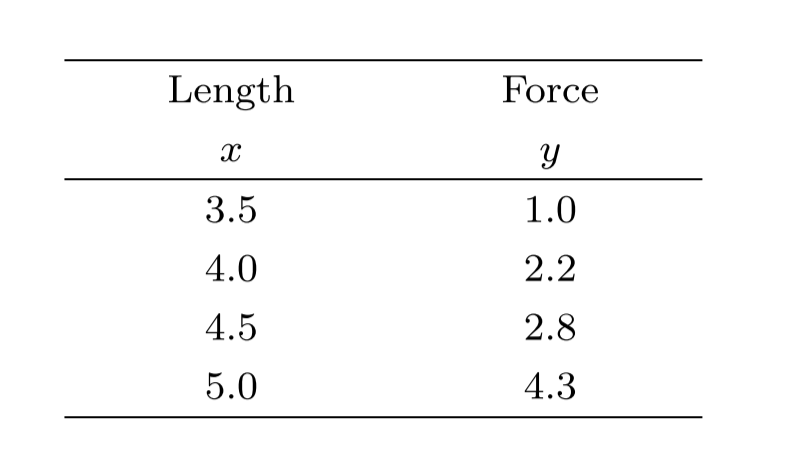
\includegraphics[width=8cm]{images/table-for-exersice-6-3-21.png}
\end{center}
\end{exercise}

\begin{proof}
\end{proof}

\begin{exercise} \label{exercise 6.3.22}
Find the \emph{minimal} solution to each of the following systems of linear equations.
\begin{enumerate}
\item
\[
    x + 2y - z = 12.
\]
\item
\[
    \sysdelim..\systeme{
        x + 2y - z = 1,
        2x + 3y + z = 2,
        4x + 7y - z = 4.
    }
\]
\item
\[
    \sysdelim..\systeme{
        x + y - z = 0,
        2x - y + z = 3,
        x - y + z = 2.
    }
\]
\item 
\[
    \sysdelim..\systeme{
        x + y + z - w =1,
        2x - y + w = 1,
        2x - y + w = 1.
    }
\]
\end{enumerate}
\end{exercise}

\begin{proof}
\end{proof}

\begin{exercise} \label{exercise 6.3.23}
Consider the problem of finding the least squares line \(y = ct + d\) corresponding to the \(m\) observations \((t_1, y_1), (t_2, y_2), ..., (t_m, y_m)\).
\begin{enumerate}
\item Show that the equation \((A^* A) x_0 = A^*y\) of \THM{6.12} takes the form of the \emph{normal equations}:
\[
    \left( \sum_{i = 1}^m t_i^2 \right) c
    + \left( \sum_{i = 1}^m t_i \right) d
    = \sum_{i = 1}^m t_i y_i
\]
and
\[
    \left( \sum_{i = 1}^m t_i \right) c + md
    = \sum_{i = 1}^m y_i.
\]
These equations may also be obtained from the error \(E\) by setting the \textbf{partial derivatives of \(E\)} with respect to both \(c\) and \(d\) equal to zero.

\item
Use the second normal equation of (a) to show that the least squares line must pass through the \emph{center of mass}, \((\overline{t}, \overline{y})\), where
\[
    \overline{t} = \frac{1}{m} \sum_{i = 1}^m t_i
    \quad \text{ and } \quad
    \overline{y} = \frac{1}{m} \sum_{i = 1}^m y_i.
\]
\end{enumerate}
\end{exercise}

\begin{proof}
\end{proof}

\begin{exercise} \label{exercise 6.3.24}
Let \(\V\) and \(\{ e_1, e_2, ... \}\) be defined as in \EXEC{6.2.23}.
Define \(\T : \V \to \V\) by
\[
    \T(\sigma)(k) = \sum_{i = 1}^{\infty} \sigma(i) \quad  \text{for every positive integer} k.
\]
Notice that the infinite series in the definition of \(\T\) \emph{converges} because \(\sigma(i) \ne 0\) for only \emph{finitely} many \(\i\).
\begin{enumerate}
\item Prove that \(\T\) is a linear operator on \(\V\).
\item Prove that for any positive integer \(n\), \(\T(e_n) = \sum_{i = 1}^n e_i.\)
\item Prove that \textbf{\(\T\) has no adjoint}.
\emph{Hint}: By way of contradiction, suppose that \(\T^*\) exists.
Prove that for any positive integer \(n\), \(\T^*(e_n)(k) \ne 0\) for infinitely many \(k\).
\end{enumerate}
\end{exercise}

\begin{proof}
\end{proof}
